\documentclass[journal,12pt,twocolumn]{IEEEtran}

\usepackage{setspace}
\usepackage{gensymb} 

\singlespacing


\usepackage[cmex10]{amsmath}

\usepackage{amsthm}


\usepackage{mathrsfs}
\usepackage{txfonts}
\usepackage{stfloats}
\usepackage{bm}
\usepackage{cite}
\usepackage{cases}
\usepackage{subfig}

\usepackage{longtable}
\usepackage{multirow}

\usepackage{enumitem}
\usepackage{mathtools}
\usepackage{steinmetz}
\usepackage{tikz}
\usepackage{circuitikz}
\usepackage{verbatim}
\usepackage{tfrupee}
\usepackage[breaklinks=true]{hyperref}
\usepackage{graphicx}
\usepackage{tkz-euclide}

\usetikzlibrary{calc,math}
\usepackage{listings}
    \usepackage{color}                                            %%
    \usepackage{array}                                            %%
    \usepackage{longtable}                                        %%
    \usepackage{calc}                                             %%
    \usepackage{multirow}                                         %%
    \usepackage{hhline}                                           %%
    \usepackage{ifthen}                                           %%
    \usepackage{lscape}     
\usepackage{multicol}
\usepackage{chngcntr}

\DeclareMathOperator*{\Res}{Res}

\renewcommand\thesection{\arabic{section}}
\renewcommand\thesubsection{\thesection.\arabic{subsection}}
\renewcommand\thesubsubsection{\thesubsection.\arabic{subsubsection}}

\renewcommand\thesectiondis{\arabic{section}}
\renewcommand\thesubsectiondis{\thesectiondis.\arabic{subsection}}
\renewcommand\thesubsubsectiondis{\thesubsectiondis.\arabic{subsubsection}}


\hyphenation{op-tical net-works semi-conduc-tor}
\def\inputGnumericTable{}                                 %%

\lstset{
%language=C,
frame=single, 
breaklines=true,
columns=fullflexible
}
\begin{document}


\newtheorem{theorem}{Theorem}[section]
\newtheorem{problem}{Problem}
\newtheorem{proposition}{Proposition}[section]
\newtheorem{lemma}{Lemma}[section]
\newtheorem{corollary}[theorem]{Corollary}
\newtheorem{example}{Example}[section]
\newtheorem{definition}[problem]{Definition}

\newcommand{\BEQA}{\begin{eqnarray}}
\newcommand{\EEQA}{\end{eqnarray}}
\newcommand{\define}{\stackrel{\triangle}{=}}
\bibliographystyle{IEEEtran}
\providecommand{\mbf}{\mathbf}
\providecommand{\pr}[1]{\ensuremath{\Pr\left(#1\right)}}
\providecommand{\qfunc}[1]{\ensuremath{Q\left(#1\right)}}
\providecommand{\sbrak}[1]{\ensuremath{{}\left[#1\right]}}
\providecommand{\lsbrak}[1]{\ensuremath{{}\left[#1\right.}}
\providecommand{\rsbrak}[1]{\ensuremath{{}\left.#1\right]}}
\providecommand{\brak}[1]{\ensuremath{\left(#1\right)}}
\providecommand{\lbrak}[1]{\ensuremath{\left(#1\right.}}
\providecommand{\rbrak}[1]{\ensuremath{\left.#1\right)}}
\providecommand{\cbrak}[1]{\ensuremath{\left\{#1\right\}}}
\providecommand{\lcbrak}[1]{\ensuremath{\left\{#1\right.}}
\providecommand{\rcbrak}[1]{\ensuremath{\left.#1\right\}}}
\theoremstyle{remark}
\newtheorem{rem}{Remark}
\newcommand{\sgn}{\mathop{\mathrm{sgn}}}
\providecommand{\abs}[1]{\left\vert#1\right\vert}
\providecommand{\res}[1]{\Res\displaylimits_{#1}} 
\providecommand{\norm}[1]{\left\lVert#1\right\rVert}
%\providecommand{\norm}[1]{\lVert#1\rVert}
\providecommand{\mtx}[1]{\mathbf{#1}}
\providecommand{\mean}[1]{E\left[ #1 \right]}
\providecommand{\fourier}{\overset{\mathcal{F}}{ \rightleftharpoons}}
%\providecommand{\hilbert}{\overset{\mathcal{H}}{ \rightleftharpoons}}
\providecommand{\system}{\overset{\mathcal{H}}{ \longleftrightarrow}}
	%\newcommand{\solution}[2]{\textbf{Solution:}{#1}}
\newcommand{\solution}{\noindent \textbf{Solution: }}
\newcommand{\cosec}{\,\text{cosec}\,}
\providecommand{\dec}[2]{\ensuremath{\overset{#1}{\underset{#2}{\gtrless}}}}
\newcommand{\myvec}[1]{\ensuremath{\begin{pmatrix}#1\end{pmatrix}}}
\newcommand{\mydet}[1]{\ensuremath{\begin{vmatrix}#1\end{vmatrix}}}
\numberwithin{equation}{subsection}
\makeatletter
\@addtoreset{figure}{problem}
\makeatother
\let\StandardTheFigure\thefigure
\let\vec\mathbf
\renewcommand{\thefigure}{\theproblem}
\def\putbox#1#2#3{\makebox[0in][l]{\makebox[#1][l]{}\raisebox{\baselineskip}[0in][0in]{\raisebox{#2}[0in][0in]{#3}}}}
     \def\rightbox#1{\makebox[0in][r]{#1}}
     \def\centbox#1{\makebox[0in]{#1}}
     \def\topbox#1{\raisebox{-\baselineskip}[0in][0in]{#1}}
     \def\midbox#1{\raisebox{-0.5\baselineskip}[0in][0in]{#1}}
\vspace{3cm}
\title{Assignment-1}
\author{G.Soujanya}
\maketitle
\newpage
\bigskip
\renewcommand{\thefigure}{\theenumi}
\renewcommand{\thetable}{\theenumi}
Download all python codes from 
\begin{lstlisting}
https://github.com/G.Soujanya/AssignmentT-1/tree/main/Assignment%201/CODES
\end{lstlisting}
%
and latex-tikz codes from 
%
\begin{lstlisting}
https://github.com/G.Soujanya/Assignment-1/tree/main/Assignment%201
\end{lstlisting}
%
\section{QUESTION NO-2.13}
\item Construct $\triangle ABC$  such that
$AB$=2.5, $BC$=6, and $AC$=6.5.Find\angle{B}
%
%
\section{SOLUTION}
Let assume, 
$AB$=c, $BC$=a, $AC$=b
 
Let
\begin{align}
\textbf{A}=\myvec{6.5 \\ 2.5},
\textbf{B}=\myvec{2.5\\ 6} ,
\textbf{C}=\myvec{6 \\ 6.5}
\end{align}
Now,
\begin{align}
\norm{\vec{A}-\vec{B}}^2 = \norm{\vec{A}}^2  =c^2=(2.5)^2=6.25
\\
\norm{\vec{B}-\vec{C}}^2 = \norm{\vec{C}}^2 =a^2=(6) ^2=36
\\
\norm{\vec{A}-\vec{C}}^2=b^2=(6.5)^2=42.25
\end{align}

From $\triangle ABC$, we use the Law of cosine:
\begin{align}
b^2=a^2+ c^2 - 2ac cos B
\\
(6.5)^2=6^2+(2.5 )^2-2*6*2.5 cos B
\\
(42.25)=36+6.25-32.5*cos B
\\
42.25-36-6.25=32.5*cos B
\\
0=32.5*cos B
\\
cos B=o
\\
 B=90
\end{align}

As we consider$\triangle ABC$  in first quadrant we consider angle {B}
\begin{align}
\therefore angle {B}=90°
\end{align}
Now, Vertices of given $\triangle ABC$ can be written as,
\begin{align}
\vec{A} = \myvec{6.5\\2.5}, \vec{B} = \myvec{2.5\\6}, \vec{C} = \myvec{6\\6.5}
\end{align}
\\
 Now, $\triangle ABC$ can be plotted using vertices $AB$ ,$BC$ and $AC$ .
\\
Plot of $\triangle ABC$:
\numberwithin{figure}{section}
\begin{figure}[ht]
    \centering
    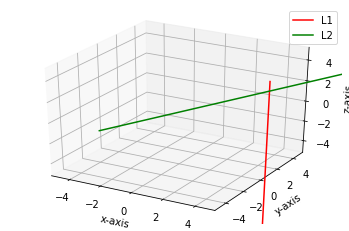
\includegraphics[width=\columnwidth]{download.png}
    \caption{ $\triangle ABC$}
    \label{fig: $\triangle ABC$}
\end{figure}
\end{document}
